\begin{figure}[htbp]
  \begin{tabular}{cc}
    \begin{minipage}{0.5\hsize}
      \centering
      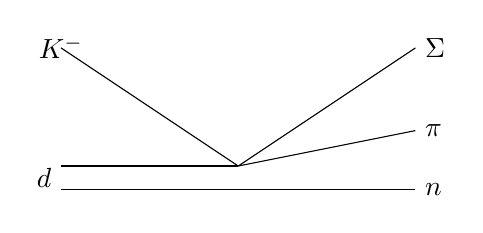
\begin{tikzpicture}[scale=1.5]
        \draw (-1.5,    1) node {$K^-$}--(0,    0);
        \draw (-1.5,    0)--(0,    0);
        \draw (-1.5, -0.2)--(0, -0.2);
        
        \node (d) at (-1.5, -0.1) [left] {$d$};

        \draw ( 1.5,  1.0) node [right] {$\Sigma$} -- (0,    0);
        \draw ( 1.5,  0.3) node [right] {$\pi$}    -- (0,    0);
        \draw ( 1.5, -0.2) node [right] {$n$}      -- (0, -0.2);
      \end{tikzpicture}
      \\
      (a) 1-step reaction
    \end{minipage}

    \begin{minipage}{0.5\hsize}
      \centering
      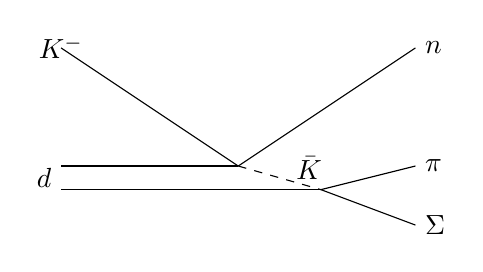
\begin{tikzpicture}[scale=1.5]
        \draw (-1.5,    1) node {$K^-$}--(0,    0);
        \draw (-1.5,    0)--(0,    0);
        \draw (-1.5, -0.2)--(0.7, -0.2);
        \node (d) at (-1.5, -0.1) [left] {$d$};

        \draw (0, 0) -- (0.7, -0.2) [dashed];
        \node (barK) at (0.6, -0.2) [above] {$\bar{K}$};

        \draw ( 1.5,  -0.5) node [right] {$\Sigma$} -- (0.7, -0.2);
        \draw ( 1.5,  -0.0) node [right] {$\pi$}    -- (0.7, -0.2);
        \draw ( 1.5,  1.0) node [right] {$n$}      -- (0,    0);
      \end{tikzpicture}
      \\
      (b) 2-step reaction
    \end{minipage}
  \end{tabular}
  \caption{Daiagrams of the $d(K^-, n)$ reaction}
  \label{fig:kd_diag}
\end{figure}
